\documentclass[11pt]{article}
\bibliographystyle{plain}
\usepackage{geometry} % see geometry.pdf on how to lay out the page. There's lots.
\usepackage{amsmath,amssymb} 
\usepackage{epsfig,epsf,subfigure}
\geometry{a4paper} 


%\documentclass{article}
%\usepackage{block}
%\usepackage{a4,psfig}

\begin{document}
\centerline{\LARGE\textbf{TMA4280 Introduction to Supercomputing}}

\vspace*{5ex}

\centerline{\Large\textbf{Problem Set 2}}

\large

\vspace*{8ex}
\centerline{Einar M. R{\o}nquist}

\vspace*{4ex}
\centerline{Spring 2012}

\subsection*{Exercise 1}

The previous supercomputer at NTNU, \texttt{njord}, was based on the 
POWER5 dual-core chip. The two processors on a single chip
each had a private L1 data cache of size 32 kB (kilobytes), 
a shared L2 cache of size 1.875 MB (megabytes), and an off-chip L3 cache 
of size 36 MB. Assume that we need to store floating 
point numbers in double precision. 
\begin{itemize}
\item How many floating point numbers 
can fit in each of the caches?
\item What is the dimension of the largest square matrix that 
we can fit in each cache? Compare this with Exercise 6  in Problem Set 1. 
\end{itemize}


\subsection*{Exercise 2}
\begin{itemize}
\item What limits are there to the speed of electronic circuits?
\item What is the maximum distance a memory unit could be from an
    arithmetic unit and still make a 100-picosecond memory access time
    conceivable?
\end{itemize}

\subsection*{Exercise 3}
Assume that we have a scalar $c$ and two vectors 
$\underline{a}$ and $\underline{b}$ of length $n$.
We consider three types of linear algebra operations: 
\begin{enumerate}
\item Add the constant $c$ to all the elements in $\underline{a}$;
\item Add the vectors $\underline{a}$ and $\underline{b}$ and store
  the result in $\underline{a}$;
\item Muliply all the elements in the vector $\underline{b}$ with the 
constant $c$ and add $\underline{a}$ to the resulting vector. 
Store the final result in $\underline{a}$.
\end{enumerate}

Below we show three FORTRAN subroutines which implement these operations
(the particular choice of high level programming language does not matter):
\begin{verbatim}
   subroutine op1 (a,c,n)
   real a(n),c
   do i=1,n
      a(i)=a(i) + c
   enddo
   return
   end
\end{verbatim}

\begin{verbatim}
   subroutine op2 (a,b,n)
   real a(n),b(n)
   do i=1,n
      a(i)=a(i) + b(i)
   enddo
   return
   end
\end{verbatim}

\begin{verbatim}
   subroutine op3 (a,b,c,n)
   real a(n),b(n),c
   do i=1,n
      a(i)=a(i) + c*b(i)
   enddo
   return
   end
\end{verbatim}

The above three routines were tested on an older supercomputer, 
a Cray T3E used at NTNU around year 2000, 
which comprised a number of DEC alpha chips 
(i.e., each processor represents a RISC architecture).
In order to check the single-processor performance, we ran a 
test program which called each of these three routines many times.
We then computed the average number of floating-point operations
for different vector lengths $n$. 
Figure 1 summarizes the performance results obtained
using a high level of compiler optimization. \\



 \begin{figure}[htbp]
  \begin{center}
    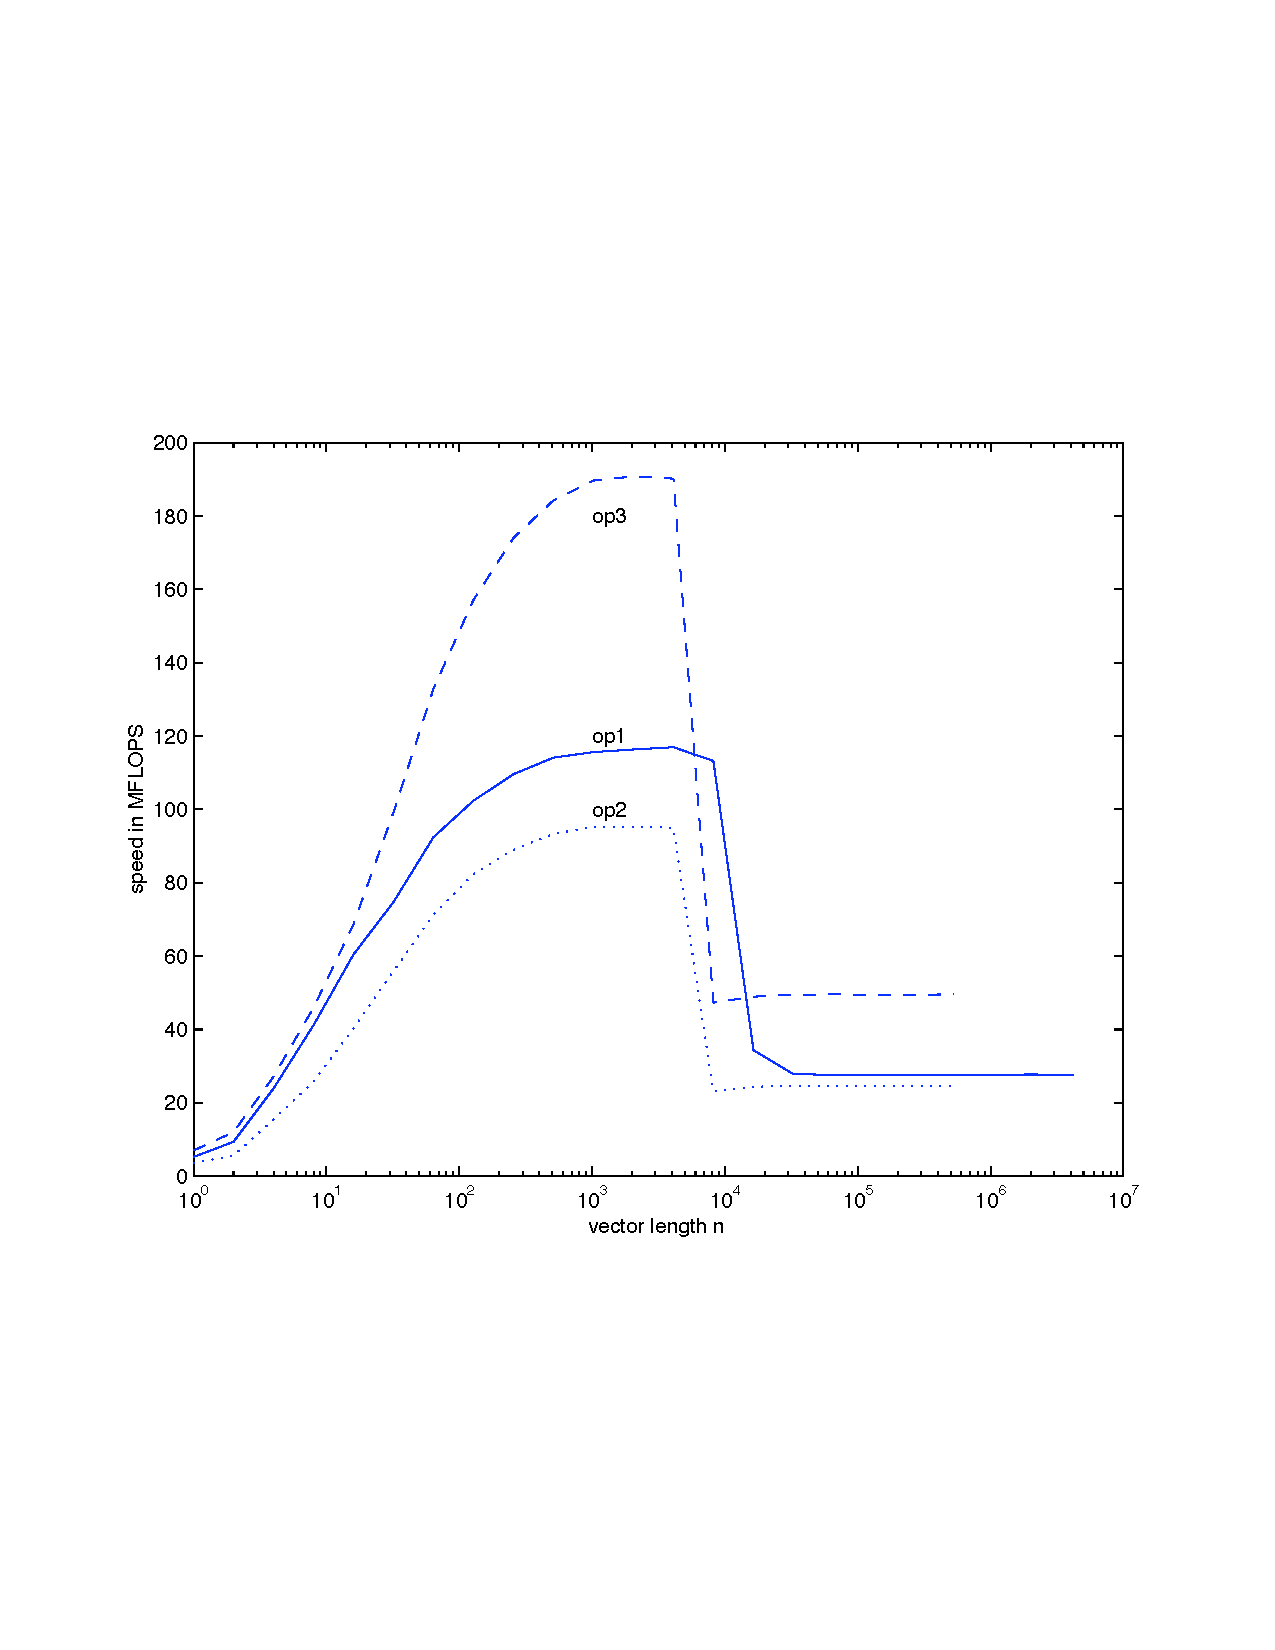
\includegraphics[scale=0.65]{ctest3}
  \end{center}
  \caption{Performance on a single alpha chip on the supercomputer \texttt{huge}. 
  This Cray T3E supercomputer was an earlier supercomputer at NTNU
  used around year 2000. }
\label{Fig1}
\end{figure}


\noindent (a) Explain these results. In particular, why does the speed of 
computation increase with $n$ for smaller vector lengths,
followed by a performance which is fairly independent of $n$?
Why is there a sudden drop in performance for a certain 
vector length? This drop was observed to happen for 
$n>4096$ for operation 2 and 3, while the drop was 
observed for $n>8192$ for operation 1. 
Why does this drop happen earlier for 
operation 2 and 3 compared to for operation 1? 
Why is the speed for operation 3 higher than for operation 1?
Why is the speed for operation 2 lower than for operation 1?\\
\\
(b) Why is it important to be aware of the memory hierarchy on 
modern computers when implementing numerical algorithms 
for scientific and technical computing?

\subsection*{Exercise 4}

Consider the vector operation 
\begin{align*}
\underline{c} = \underline{a} + \underline{b},
\end{align*}
where $\underline{a}$, $\underline{b}$, and $\underline{c}$ 
are vectors of length $n$. One way to implement this operation is: 
\begin{verbatim}
                          for i=1,n
                               c(i) = a(i) + b(i)
                          end
\end{verbatim}

In order to optimize the expected performance, we want to make 
sure that the vector elements are stored next to each other 
in the main memory in the following sequence: 
$\ldots, a(i), b(i), c(i), a(i+1), b(i+1), c(i+1), \ldots$. 
\begin{itemize}
\item Why could this way of storing the data be advantageous?
\item How would you realize this in C and/or in FORTRAN?
\item Do you think it matters much whether we store the vector elements
in the above sequence, in particular, compared to just allocating the vectors 
$\underline{a}$, $\underline{b}$, $\underline{c}$ separately, 
i.e., each vector is stored contiguously in main memory?
\end{itemize}

\subsection*{Coding task}

Implement a program in C/Fortran which performs the following operations:
\[
  \begin{split}
    \underline{x} &= \underline{a} + \gamma\underline{b} \\
    \underline{y} &= \underline{a} + \underline{A}\underline{b} \\
    \alpha &= \underline{x}^T\underline{y}
  \end{split}.
\]

You can use any compatible vectors and matrices you see fit (e.g. random), and $\gamma$
should be taken from the command line.

\end{document}



\subsection*{Exercise 4 from Problem set 1 in 2004 !!!!!!!!!!!!!!!}

The supercomputer you will be using, gridur, comprises the 
MIPS processor R14000. Each processor has two caches for 
data, an L1 cache of size 32 kB (kilobytes) and an L2 cache 
of size 8MB (megabytes). How many floating point numbers 
can fit in each of the caches assuming double precision?
What is the dimension of the largest square matrix that 
we can fit in each cache? You can assume that the matrix
elements are floating point numbers in double precision.


\subsection*{Exercise 1}
\begin{enumerate}
\item What limits are there to the speed of electronic circuits?
\item What is the maximum distance a memory unit could be from an
    arithmetic unit and still make a 100-picosecond memory access time
    conceivable?
\end{enumerate}
